\chapter{Antennas} % (fold)
\label{cha:antennas}

\section{Radio Link} % (fold)
\label{sec:radio_link}


\subsection{Link Budget} % (fold)
\label{sub:link_budget}

\begin{figure}[h]
	\centering
	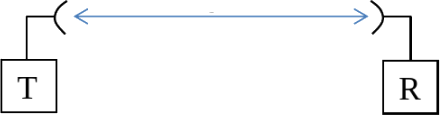
\includegraphics[scale=0.6]{Immagini/link}
	
	\caption{Simplified scheme of a Radio Link}
	\label{fig:link}
\end{figure}

Supposing to have a Radio Link as in Figure~\ref{fig:link} between 2 Antennas at a certain relative distance R the link budget may be evaluated by means of the \textbf{Friis equation} which at the end leds to a simple analitical expression for the receiving power:

\begin{equation}	
P_{r|_{dB}} = P_{t|_{dB}} - 10 \log{frac{\lambda}{4\pi R}} + G_{t|_{dB}} + G_{r|_{dB}} 
\end{equation}

in which:

\begin{itemize}
	\item $P_{r|_{dB}}$ is the effective power received by the antenna.
	\item $P_{t|_{dB}}$ is the overall transmitted power of the TX side.
	\item $G_{r|_{dB}}$ is the gain of the receiving antenna.
	\item $G_{t|_{dB}}$ is the gain of the transmitting antenna.
\end{itemize}

while the term $20\log{ \frac{\lambda}{4 \pi R} }$ stands for the free space losses.
Note from a practical point of view there as at least a couple of DoF in the design flow to obtain a certain receiving power.

% subsection link_budget (end)

\subsection{Antennas' Gain} % (fold)
\label{sub:antennas_gain}





% subsection antennas_gain (end)


\subsection{Equivalent Temperature} % (fold)
\label{sub:equivalent_temperature}

\begin{figure}[h]
	\centering
	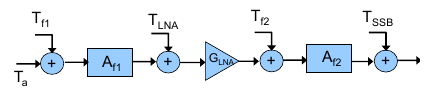
\includegraphics[scale=1]{Immagini/Teq}
	
	\caption{General structure of a noisy receiving chain}
	\label{fig:Teq}
\end{figure}


Supposing to have a receiving chain as in Figure\footnote{note that here $A_x$ stands for an attenuation $= \frac{1}{Gain}$ and G stands for a Gain}~\ref{fig:Teq} we may want to rappresent the system with noiseless components and an input referred noise considering all contribution.
This could be very usefull beacuse using this model the Signal-to-Noise Ratio evalutation turns out to be extremly simple, while we can just compare the receiving power with the overall noise directly at the input port.

To get an $T_{equivalent}$ we have to refer at the input any additional noise by dividing it by the Gain from to input to the point where the noise is injected.

At the end for the example in figure we get:

\begin{equation}
	T_{sys}=T_{eq}= T_a + T_{f1} + T_{LNA} A_{f1}+ T_{f2} \frac { A_{f1} } {G_{LNA}} + T_{SSB} \frac { A_{f1} A_{f2} } {G_{LNA}}
\end{equation}

With the same concept we may find the \textit{Output Referred Noise} $T_out$ by simply applyng the relative transfer function at each noise to the ouput:

\begin{equation}
	T_out = T_a\frac {G_{LNA}} {A_{f1} A_{f2} } + T_{f1}\frac { G_{LNA}} {A_{f1}A_{f2}} + T_{LNA}\frac{G_{LNA}}{A_{f2}}+ T_{f2}\frac{1}{A_{f2}} + T_{SSB} 
\end{equation}

and to get $T_{eq}$ we may divide $T_{out}$ by the noiseless gain $\frac{G_{LNA}}{A_{f1}A_{f2}}$

\begin{equation}
	T_{eq}=\frac{T_out}{\frac{G_{LNA}}{A_{f1}A_{f2}}}
\end{equation}

after some algebra it's clear that the two different approaches are absolutely equivalent.





% subsection equivalent_temperature (end)


% section radio_link (end)

% chapter antennas (end)